% $Id$
% ---------------------------------------------------------------------------
%
%  This is part of the SIGI.
%  Copyright (C) 2008 Interlegis
%  See the file relatorio.tex for copying conditions.
%

\section{Modelo de dados}
\label{sec:modelo}

\subsection{Diagrama de Entidade e Relacionamento (figura \ref{fig:er})}
\begin{figure}[p]
  \centering
  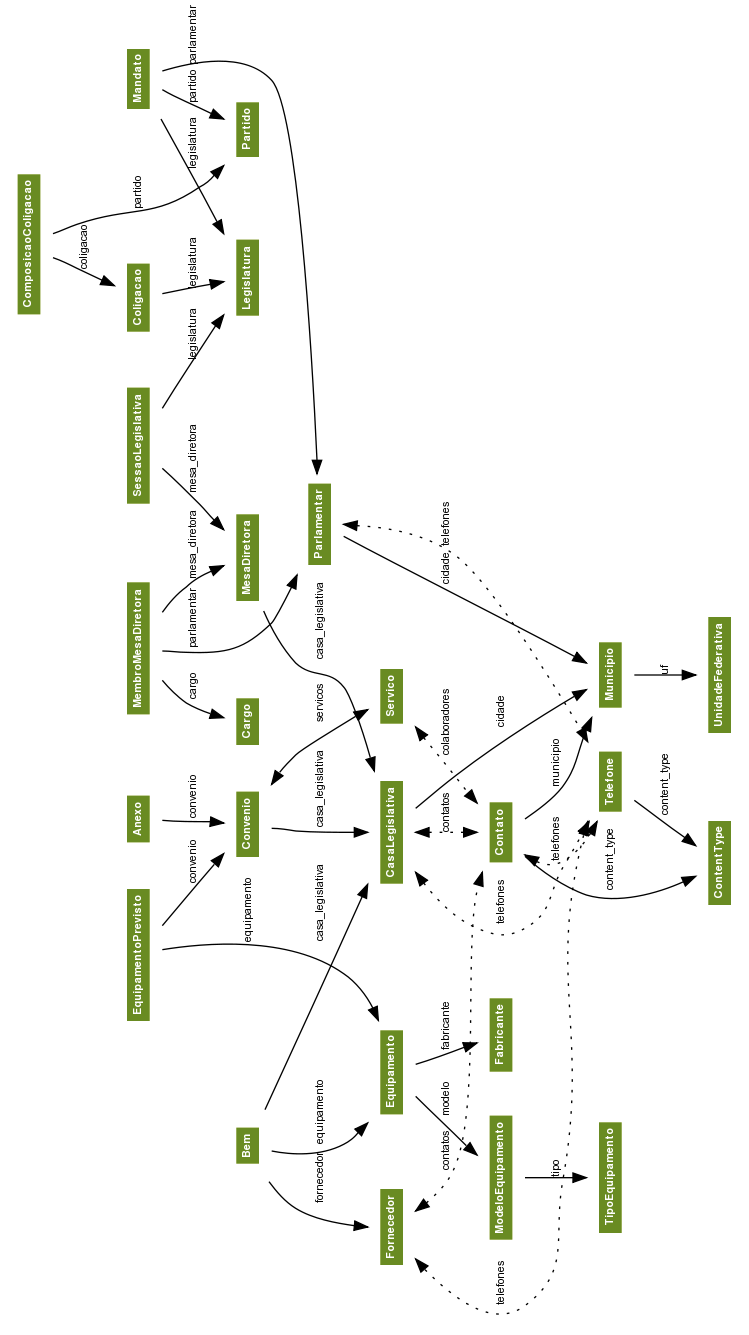
\includegraphics[width=120mm]{../imagens/er.png}
  \caption{Diagrama de Entidade e Relacionamento do SIGI}
  \label{fig:er}
\end{figure}

\subsection{Diagrama de Classes}
\subsubsection{Aplicação sigi.apps.casas (figura \ref{fig:casas})}
\begin{figure}[h]
  \centering
  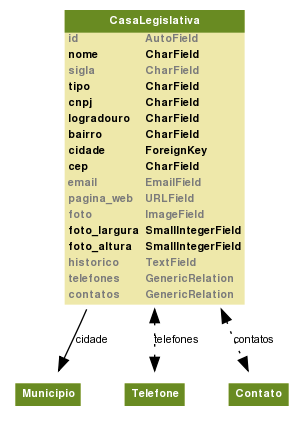
\includegraphics[width=60mm]{../imagens/casas.png}
  \caption{Diagrama de Classes da aplicação sigi.apps.casas}
  \label{fig:casas}
\end{figure}

\subsubsection{Aplicação sigi.apps.contatos (figura \ref{fig:contatos})}
\begin{figure}[h]
  \centering
  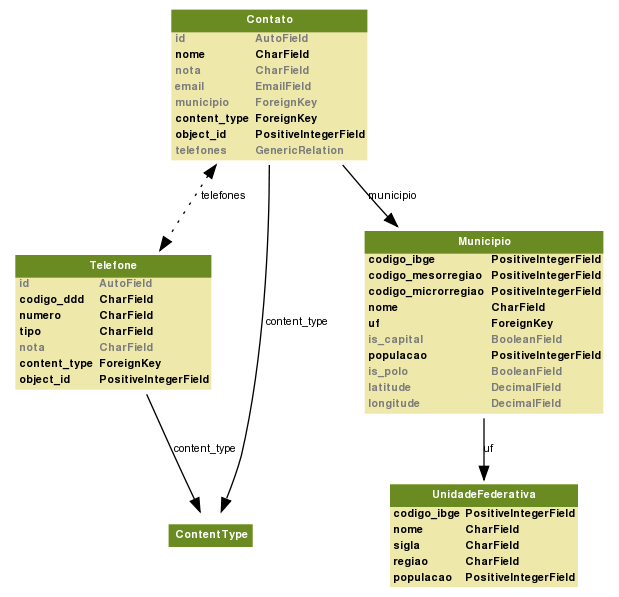
\includegraphics[width=120mm]{../imagens/contatos.png}
  \caption{Diagrama de Classes da aplicação sigi.apps.contatos}
  \label{fig:contatos}
\end{figure}

\subsubsection{Aplicação sigi.apps.convenios (figura \ref{fig:convenios})}
\begin{figure}[h]
  \centering
  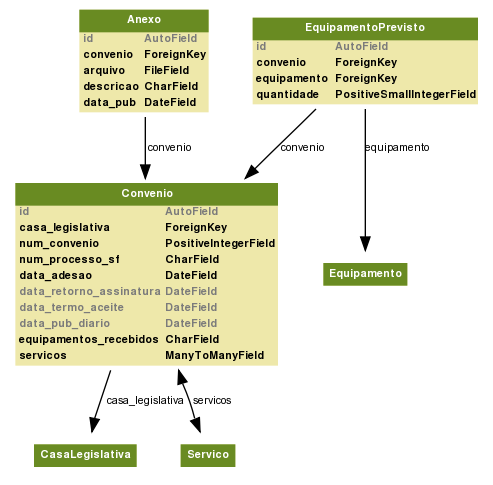
\includegraphics[width=100mm]{../imagens/convenios.png}
  \caption{Diagrama de Classes da aplicação sigi.apps.convenios}
  \label{fig:convenios}
\end{figure}

\subsubsection{Aplicação sigi.apps.inventario (figura \ref{fig:inventario})}
\begin{figure}[h]
  \centering
  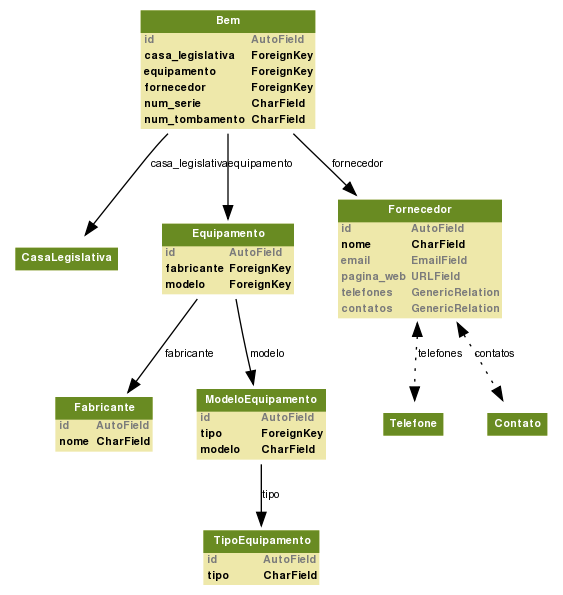
\includegraphics[width=120mm]{../imagens/inventario.png}
  \caption{Diagrama de Classes da aplicação sigi.apps.inventario}
  \label{fig:inventario}
\end{figure}

\subsubsection{Aplicação sigi.apps.mesas (figura \ref{fig:mesas})}
\begin{figure}[h]
  \centering
  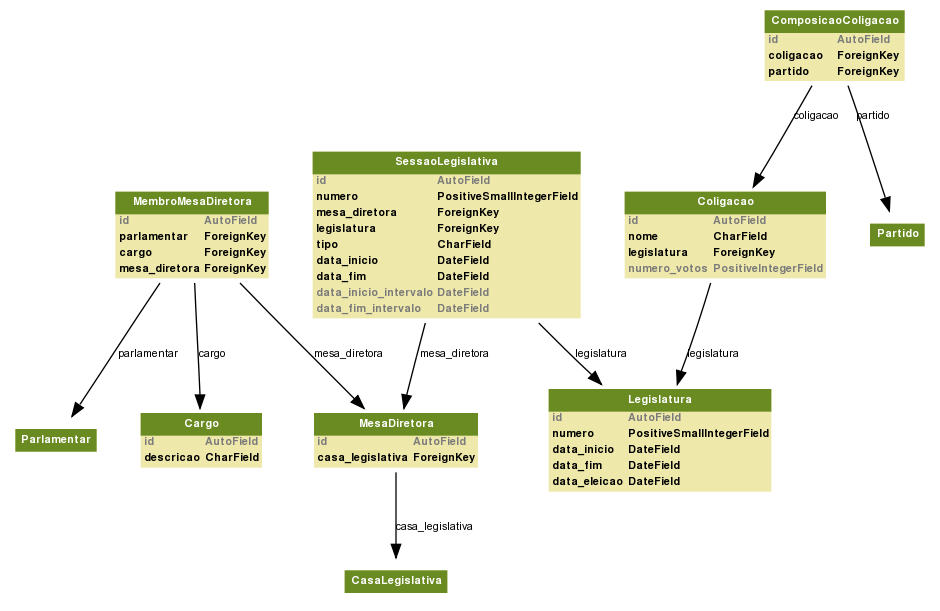
\includegraphics[width=145mm]{../imagens/mesas.png}
  \caption{Diagrama de Classes da aplicação sigi.apps.mesas}
  \label{fig:mesas}
\end{figure}

\subsubsection{Aplicação sigi.apps.parlamentares (figura \ref{fig:parlamentares})}
\begin{figure}[h]
  \centering
  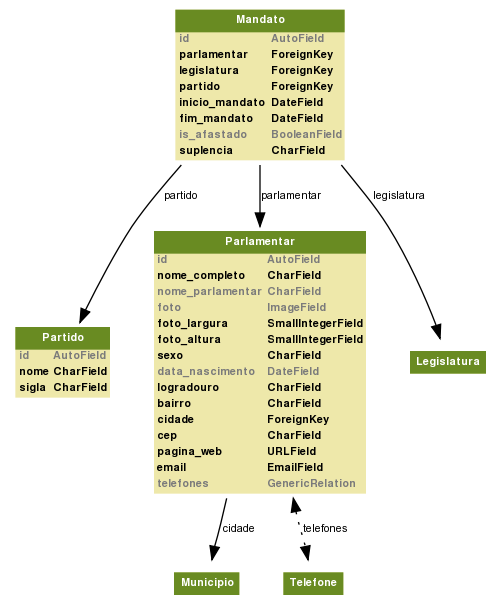
\includegraphics[width=100mm]{../imagens/parlamentares.png}
  \caption{Diagrama de Classes da aplicação sigi.apps.parlamentares}
  \label{fig:parlamentares}
\end{figure}

\subsubsection{Aplicação sigi.apps.servicos (figura \ref{fig:servicos})}
\begin{figure}[h]
  \centering
  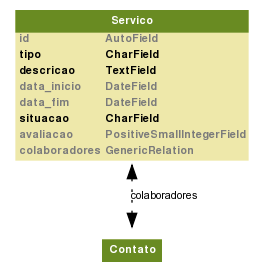
\includegraphics[width=60mm]{../imagens/servicos.png}
  \caption{Diagrama de Classes da aplicação sigi.apps.servicos}
  \label{fig:servicos}
\end{figure}

%
% Local variables:
%   mode: flyspell
%   TeX-master: "relatorio.tex"
% End:
%
